\subsubsection{Définition}
Nous avons commencé nos recherches en nous intéressant en premier lieu aux moyens d'échanges les plus répandus. 
Cela nous a mené vers les plate-formes d'échanges centralisé ou \acrshort{cex}. 
Ce sont des plate-formes, pouvant prendre la forme d'applications web, qui permettent aux utilisateurs d'acheter, de vendre ou d'échanger des \gls{actif}s numériques contre d'autres \gls{actif}s numériques ou en monnaies fiduciaires. 
Ces plate-formes peuvent opérer sur des \textit{\gls{blockchain}s} publiques ou être dédiées à une utilisation en interne. 
Elles sont dites centralisées car elles sont gérées par une entreprise ou une organisation hiérarchisée qui contrôle les transactions et les fonds des utilisateurs.
Ces plate-formes sont donc considérées comme des tiers de confiance et agissent en tant qu'intermédiaires entre les acheteurs et les vendeurs en assurant la sécurité, la liquidité et la rapidité des transactions.
C'est la solution la plus utilisée dans le secteur des \gls{actif}s numériques, elles offrent très souvent une certaine variété de services tels que le prêt et/ou le \textit{stacking} \footnote{Stacking : Action de verrouiller des jetons en vue de recevoir des récompenses \cite{defStack}}.
Elles proposent également un large éventail de cryptomonnaies disponibles.

\subsubsection{Inconvénients et risques}
Nous avons pu tout de même relever certains inconvénients et certains risques pour les utilisateurs liés à l'utilisation de ces plate-formes. 
Tout d'abords, les utilisateurs doivent confier leurs fonds et leurs données à un tier en qui ils doivent avoir confiance. 
Cela peut exposer les utilisateurs à de la fraude, du vol ou encore du piratage si les plate-formes présentent des failles de sécurité. \\
Ensuite, ces plate-formes peuvent être victimes de pannes ou de saturation du réseau pouvant entraîner des retards, des pertes de transactions ou encore du déni de service bloquant ainsi l'accès aux \gls{actif}s des utilisateurs. 
Finalement, ces plate-formes sont soumises à la réglementation et à la surveillance des autorités financières, limitant leur accessibilité dans certains pays ou régions. 
Ce point signifie aussi que les \gls{actif}s de l'utilisateurs sont traçables par les autorités. 


\subsubsection{Fonctionnement}
\begin{figure}[h!]
    \centering
    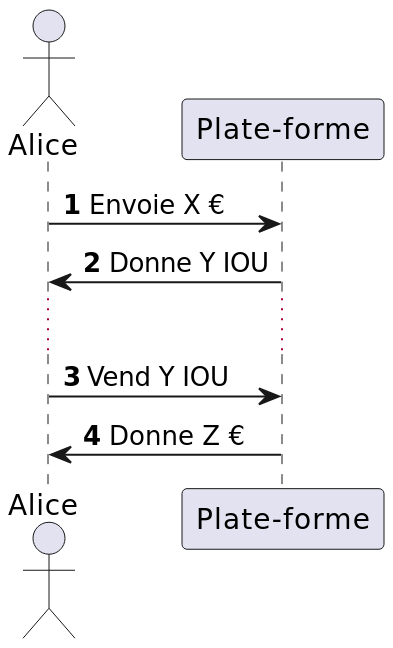
\includegraphics[scale=0.2]{centralisation/Achat-Vente.png}
    \label{fig:simplifiedcex}
    \caption{Échange d'un jeton en Euros}
\end{figure}
Ces plate-formes fonctionnent sur le principe de l'\textit{order book method} (méthode du carnet d'ordre\cite{orderBook}), une modélisation des ordres d'achats et de vente des jetons.
Un ordre étant une demande d'un utilisateur visant à réaliser une opération à un prix et une quantité donnée. 
Cette méthode comprend deux parties: l'offre et la demande. L'offre regroupe les ordres d'achats émis par des utilisateurs sur la plate-forme et la demande, les ordres de vente.
Lors d'un dépôt, l'utilisateur s'étant au préalable enregistré sur la plate-forme, il va déposer les fonds souhaités dans un porte monnaie. 
La plate-forme va ensuite crée un \textit{\acrshort{iou}}\footnote{I Owe You, c'est la dette de la plate-forme envers l'utilisateur permettant de bloquer la valeur de la monnaie déposée par l'utilisateur\cite{IOU}} 
ce dernier sera échangé contre le crypto-\gls{actif} souhaité lors d'un échange ou d'une vente. \\ 

Dans le cadre des échanges inter-\gls{blockchain}s, les plate-formes d'échanges utilisent des \textit{bridges} reliant les différentes \textit{\gls{blockchain}s}. 
Ces protocoles seront explicités dans la partie suivante.
Cependant, nous n'avons pas pu trouver de plus amples explications quant aux fonctionnements des plate-formes, notamment les protocoles précis utilisés lors des échanges. 
Les documentations disponibles pour les plateformes d'échanges étant à destination des utilisateurs finaux. 


